\section{Introduction} \label{sec:introduction}
    \IEEEPARstart{M}{otion}

% \vspace{-0.3cm}

\section{Methods} \label{sec:methods}
    \subsection{XCAT Volume Generation} \label{sec:xcat_volume_generation}
        
        
    % \vspace{-0.3cm}
    
    \subsection{Evaluation} \label{sec:evaluation}
        

% \vspace{-0.3cm}

\section{Results} \label{sec:results}
    % \begin{figure}
        % \vspace{-0.0cm}
        
    %     \centering
        
    %     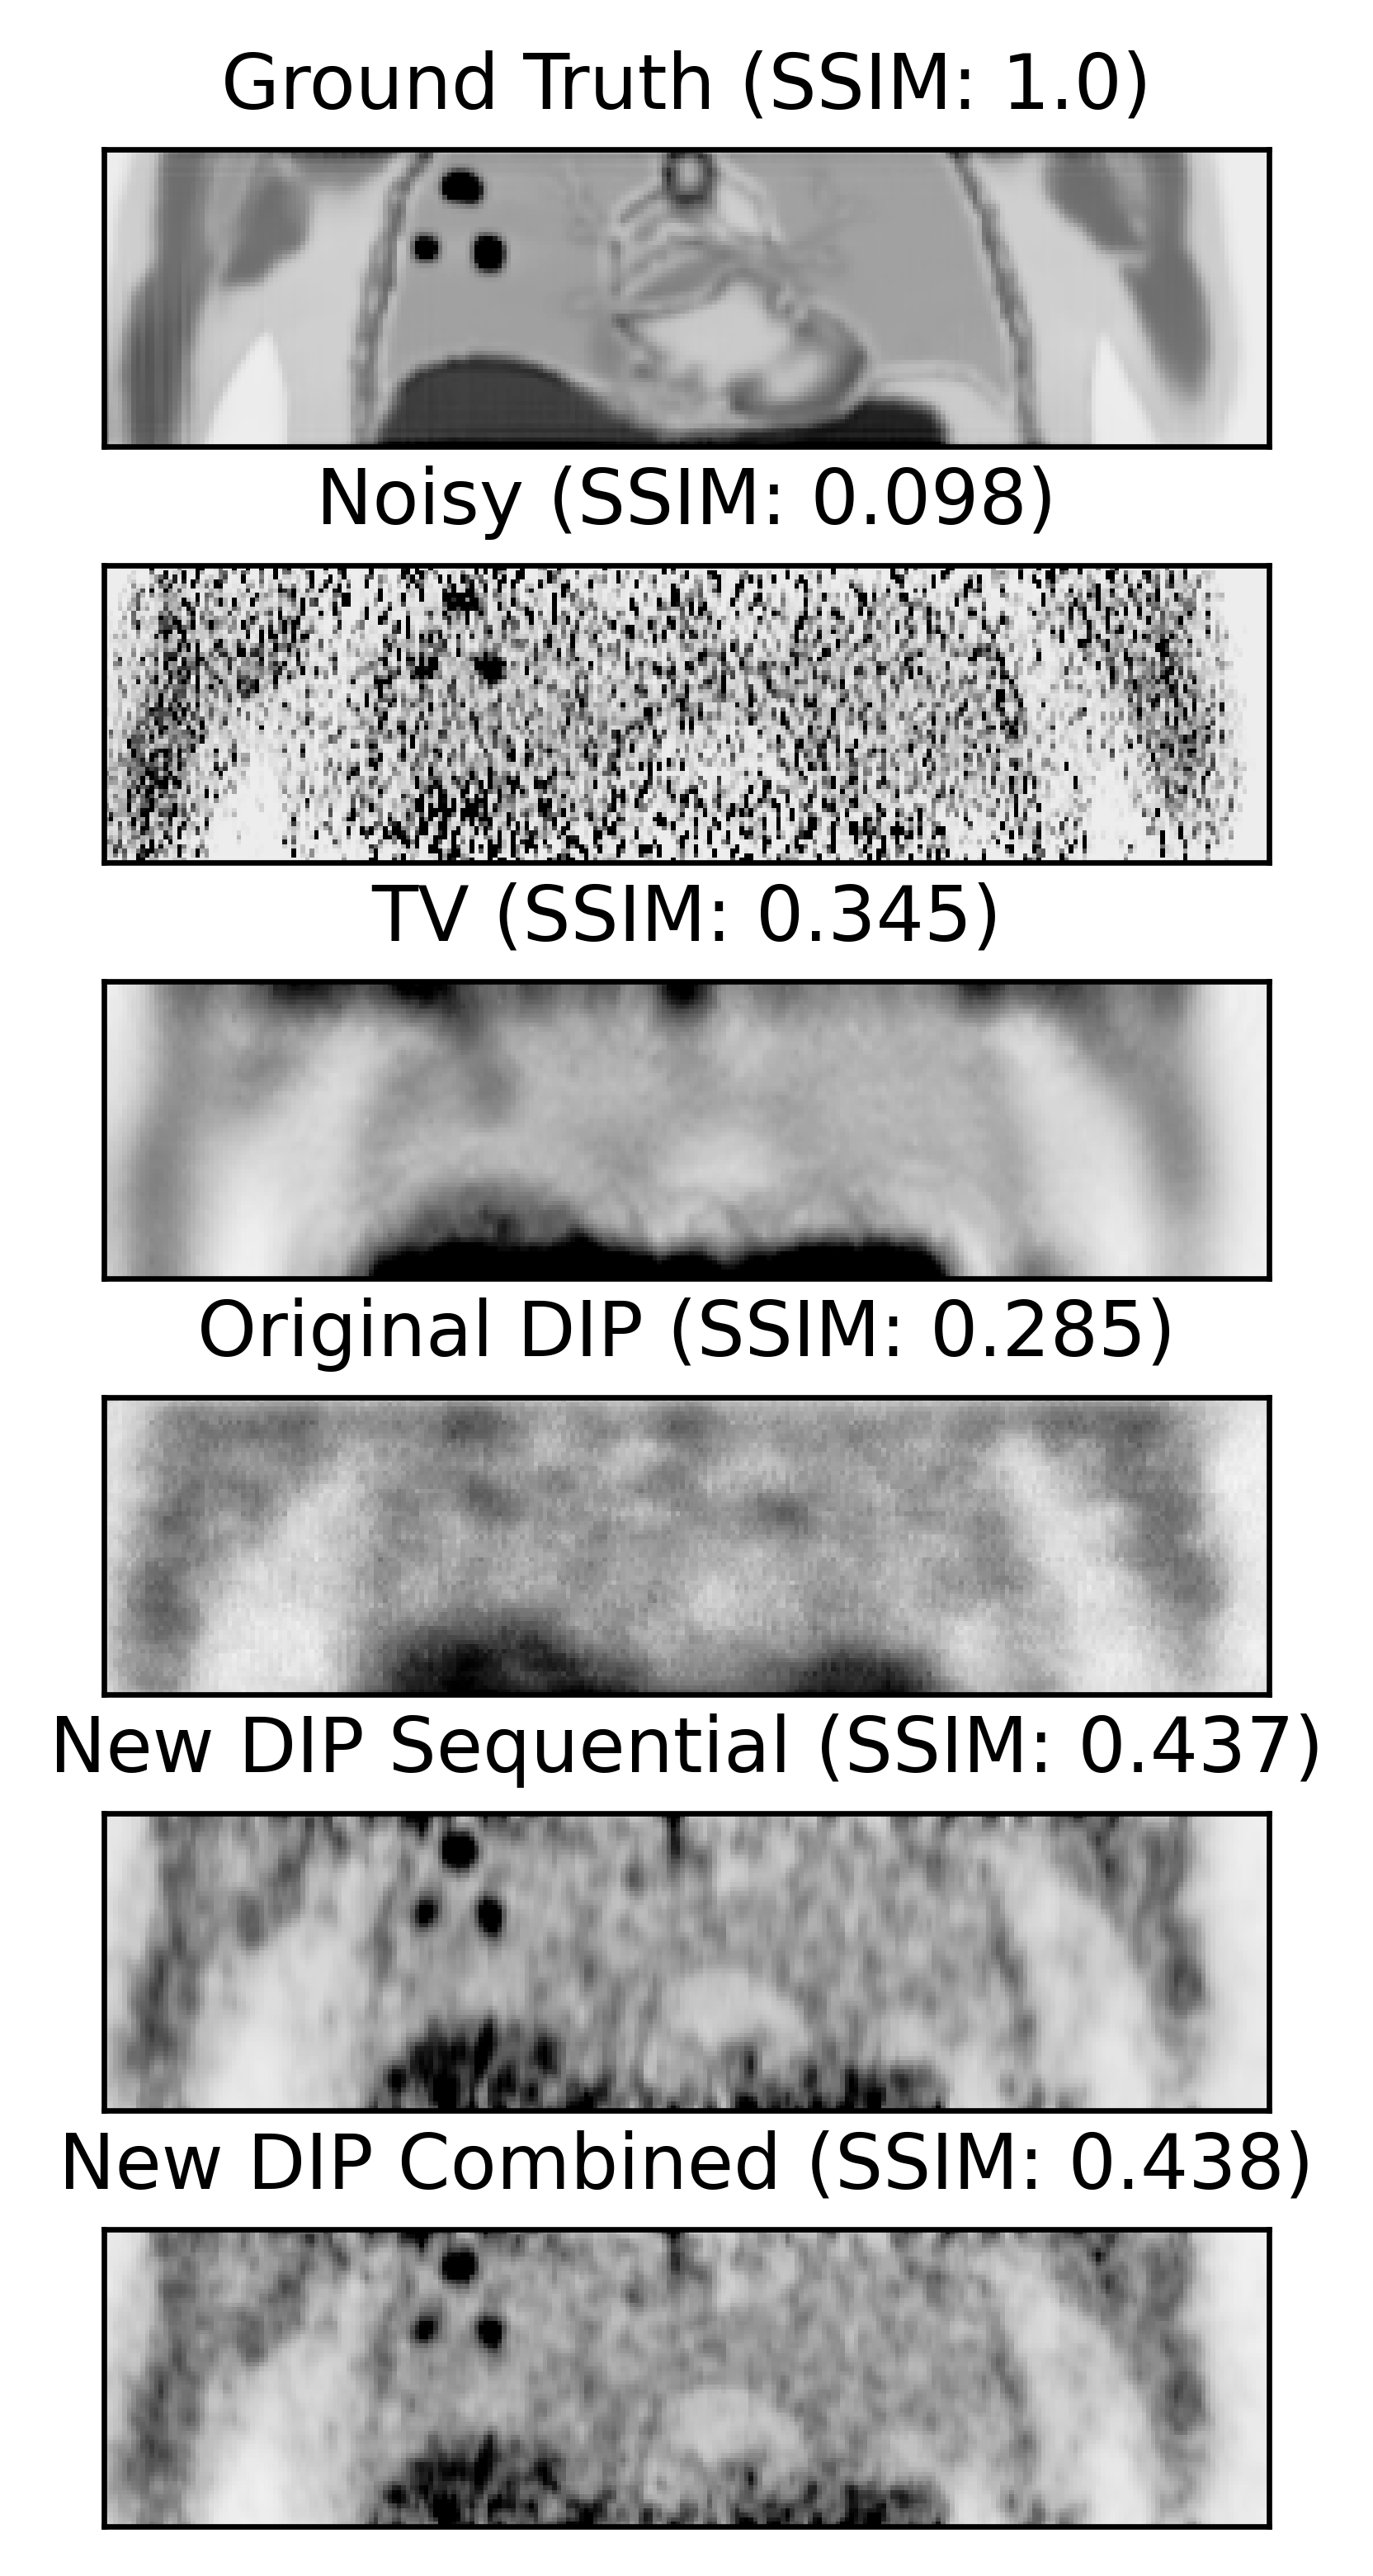
\includegraphics[width=1.0\linewidth]{figures/visual_analysis.png}
        
        % \vspace{-0.3cm}
        
    %     \captionsetup{singlelinecheck=false, justification=centering}
    %     \caption{First column contains \gls{AC} \gls{MC} reconstructions and the second column contains the result of applying the final \gls{MC} on the original XCAT images (for easier assessment of the accuracy of the estimated \glss{DVF}); ungated static \gls{CT}, ungated \gls{AV-CCT}, pair-wise, pair-wise \gls{MM}, group-wise, group-wise \gls{MM}. Colour map ranges are consistent for all images in each column.}
        
    %     \label{fig:visual_analysis}
        
        % \vspace{-0.3cm}
    % \end{figure}
    
    

% \vspace{-0.3cm}

\section{Discussion and Conclusions} \label{sec:discussion_and_conclusions}
    
    